\documentclass[12pt,a4paper]{article}

\usepackage[utf8]{inputenc}
\usepackage[T2A]{fontenc}
\usepackage[ukrainian]{babel}

\usepackage{geometry}
\geometry{left=2cm,right=2cm,top=2cm,bottom=2cm}

\usepackage{graphicx}
\usepackage{array,multirow}
\usepackage{booktabs}
\usepackage{caption}

\usepackage{enumitem}

\usepackage{amsmath}
\usepackage{xcolor}

\usepackage{minted}

\usemintedstyle{vs} % або monokai / vs / colorful
\setminted{linenos, breaklines, frame=single, fontsize=\small}

\usepackage{hyperref}

\begin{document}

    \begin{titlepage}

        % Картинка шапки (по центру, з відступом від верху)
        \begin{center}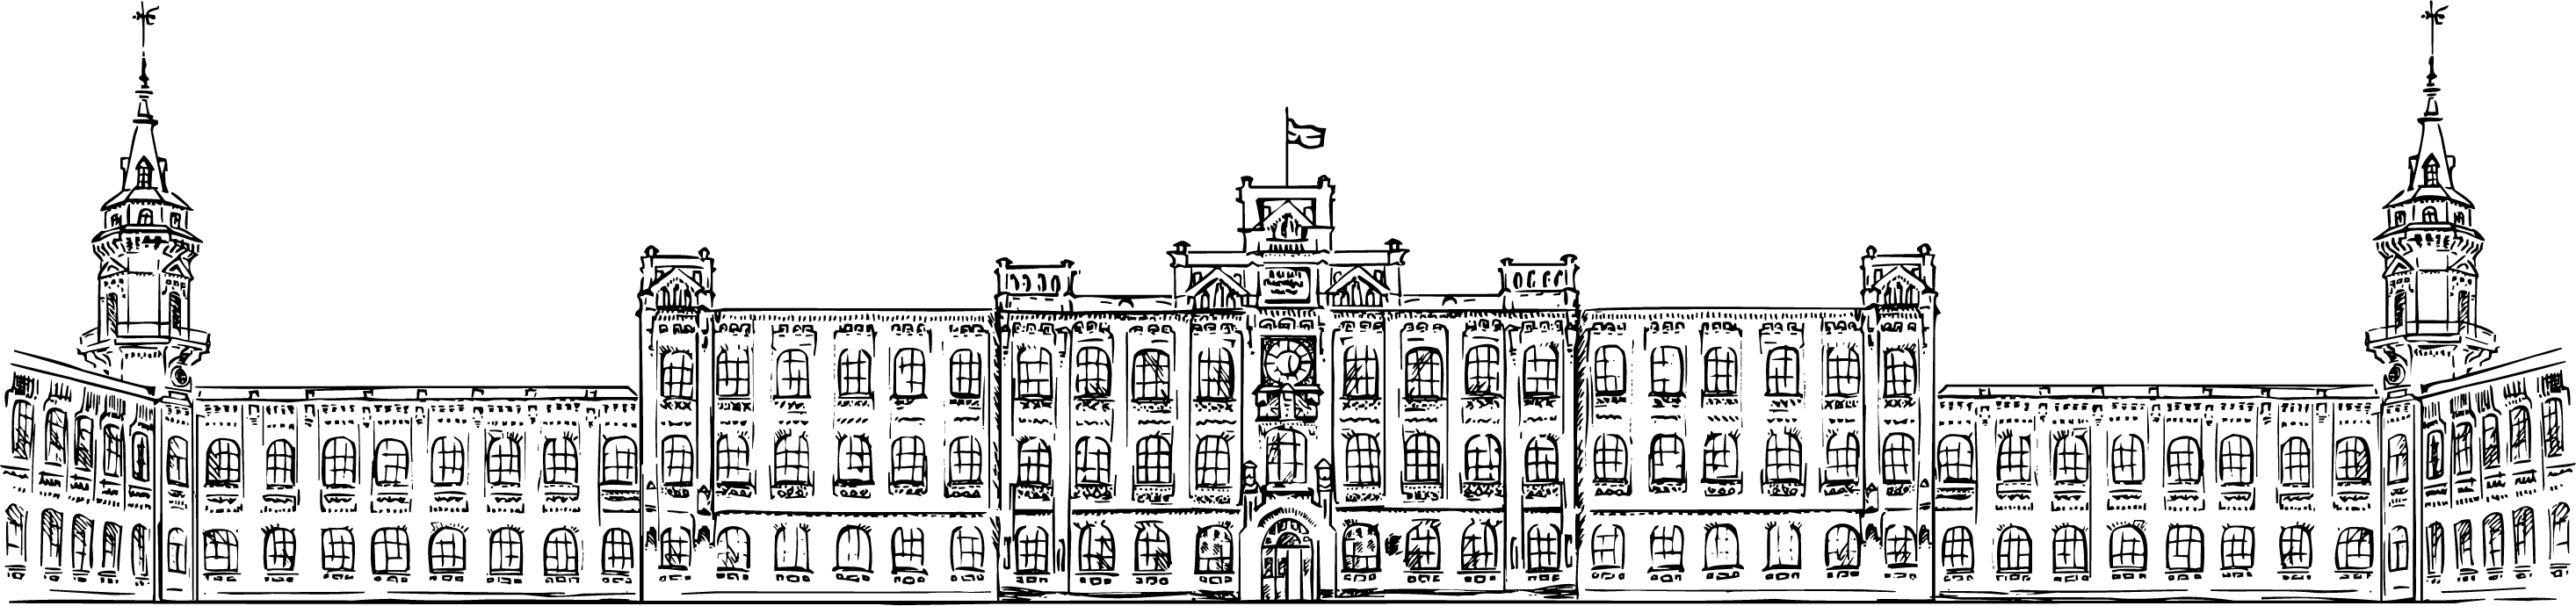
\includegraphics[width=0.7\textwidth]{../../../../TITLES/letterhead.png}\end{center}

        \begin{center}
            \large Національний технічний університет України\\
            «Київський політехнічний інститут імені Ігоря Сікорського»\\[1em]
            Факультет інформатики та обчислювальної техніки\\
            Кафедра обчислювальної техніки
        \end{center}

        \vfill

        \begin{center}
            \textbf{\LARGE Вступ до операційної системи Linux. Курсова робота}\\[1.5em]
            \textbf{\Large Завдання №4}\\[1em]
            «Вивчення CI/CD інстументів»
        \end{center}

        \vfill

        \begin{flushright}
            Виконав: студент 2 курсу ФІОТ, гр. ІО-41\\
            \textit{Давидчук А.~М.}\\[1em]
            Перевірив: \textit{Нікольський С.~С.}
        \end{flushright}

        \vfill

        \begin{center}Київ --- 2025\end{center}

    \end{titlepage}

    % Основний документ:

    \setlength{\parindent}{0em}

    \textbf{\underline{Тема:}} «Вивчення CI/CD інстументів»

    \vspace{1em}

    \textbf{\underline{Мета:}} навчитись користуванню інструментів CI/CD інструментів на основі Jenkins.

    \vspace{1em}

    \begin{center} \textbf{\Large Практична частина} \end{center}

    

    \textbf{\underline{Висновок:}}

\end{document}